\documentclass[9pt,twoside,lineno]{pnas-new}
% Use the lineno option to display guide line numbers if required.

\templatetype{pnassupportinginfo}
% \readytosubmit %% Uncomment this line before submitting, so that the instruction page is removed.

\usepackage{bbm}
\usepackage{algorithm}
\usepackage[noend]{algpseudocode}
\graphicspath{{figures/}}
\DeclareMathOperator{\Tr}{Tr}

\title{Learning complex models with invertible neural networks: a likelihood-free Bayesian approach}
\author{Stefan T. Radev, Ulf K. Mertens, Andreas Voss, Lynton Ardizzone, and Ullrich Köthe}
\correspondingauthor{Stefan Radev.\\E-mail: stefan.radev@psychologie.uni-heidelberg.de}

\begin{document}


\maketitle

%% Adds the main heading for the SI text. Comment out this line if you do not have any supporting information text.
\SItext


\section*{Results}


\subsection*{Performance metrics}

In the following, the computation of the performance metrics used throughout the main text is detailed.

\subsubsection*{Normalized Root Mean Squared Error}
The normalized root mean squared error (NRMSE) between a sample of true parameters $\{\theta^{(i)}\}_{i=1}^{n}$ and a sample of estimated parameters $\{\hat{\theta}^{(i)}\}_{i=1}^{n}$ is given by:
\begin{align*}
NRMSE = \sqrt{\sum_{i=1}^{n}\frac{\left(\theta^{(i)}-\hat{\theta}^{(i)}\right)^{2}}{\theta_{max}- \theta_{min}}} \numberthis \label{eqn:1}
\end{align*}
Due to the normalization factor $\theta_{max}-\theta_{min}$, the NRMSE is scale-independent, and thus suitable for comparing the recovery across parameters having different numerical ranges. The NRMSE is zero when the estimates are exactly equal to the true values.
\subsubsection*{Coefficient of Determination }
The coefficient of determination $R^{2}$ gives the proportion of variance in a sample of true parameters $\{\theta^{(i)}\}_{i=1}^{n}$ that is "explained" by a sample of estimated parameters $\{\hat{\theta}^{(i)}\}_{i=1}^{n}$. It is computed as:
\begin{align*}
R^{2} = 1 - \sum_{i=1}^{n}\frac{\left(\theta^{(i)}-\hat{\theta}^{(i)}\right)^{2}}{\left(\theta^{(i)}-\bar{\theta}^{(i)}\right)^{2}} \numberthis \label{eqn:2}
\end{align*}
where $\bar{\theta}$ denotes the mean of the true parameter samples. When $R^{2}$ equals $1$, it means that the estimates are perfect reconstructions of the true parameters.

\subsubsection*{Kullback-Leibler Divergence} The Kullback-Leibler divergence ($D_{KL}$) quantifies the increase in entropy incurred by approximating a target probability distribution $P$ with a distribution $Q$. Its general form for absolutely continuous distributions is given by
\begin{align*}
D_{KL}(P||Q) = \int_{-\infty}^{\infty} p(x)\log\frac{p(x)}{q(x)} dx \numberthis \label{eqn:3}
\end{align*}
where $p$ and $q$ denote the pdfs of $P$ and $Q$. In the case where $P$ and $Q$ are both multivariate Gaussian distributions, the KL divergence can be computed in closed form \cite{hershey2007approximating}:
\begin{align*}
D_{KL}(P||Q) = \frac{1}{2}\left[\log\frac{\det\boldsymbol{\Sigma}_{q}}{\det\boldsymbol{\Sigma}_{p}} + \Tr(\boldsymbol{\Sigma}_{q}^{-1}\boldsymbol{\Sigma}_{p}) - d + (\boldsymbol{\mu}_{p} - \boldsymbol{\mu}_{q})^{T}\boldsymbol{\Sigma}_{q}^{-1}(\boldsymbol{\mu}_{p} - \boldsymbol{\mu}_{q})\right] \numberthis \label{eqn:4}
\end{align*}
where $\boldsymbol{\Sigma}_{p}$ and $\boldsymbol{\Sigma}_{q}$ denote the covariance matrices of $p$ and $q$, $\boldsymbol{\mu}_{p}$ and $\boldsymbol{\mu}_{q}$ the respective mean vectors, and $d$ the number of dimensions of the Gaussian. In the case of diagonal Gaussian distributions, Eq.\ref{eqn:4} reduces to:
\begin{align*}
D_{KL}(P||Q) = \sum_{i=1}^d\left(\log\frac{\sigma_{q,i}}{\sigma_{p,i}} + \frac{\sigma_{p,i}^{2} + (\mu_{q,i} - \mu_{p,i})^{2}}{2\sigma_{q,i}^{2}} - \frac{1}{2} \right) \numberthis \label{eqn:5}
\end{align*}
Even though the KL divergence is not a proper distance metric, as it is not symmetric in its arguments, it can be used to quantify the error of approximation and serve as a metric for comparing different methods. 

\subsubsection*{Simulation-Based Calibration}
Simulation-based calibration is a recently proposed method for validating the accuracy of posterior samples generated by a Bayesian sampling method \cite{talts2018validating}. It is based on the so called \textit{self-consistency} of the Bayesian joint distribution. Given a sample from the prior distribution $\tilde{\theta} \sim p(\theta)$ and a sample from the data-generating process $\tilde{x} \sim p(x|\tilde{\theta})$, one can integrate $\tilde{\theta}$ and $\tilde{x}$ out of the Bayesian joint distribution to recover back the prior of $\theta$:
\begin{align*}
p(\theta) &= \int p(\theta,\tilde{\theta},\tilde{x})d\tilde{x}d\tilde{\theta} \numberthis  \label{eqn:6} \\
&= \int p(\theta,\tilde{x}|\tilde{\theta})p(\tilde{\theta})d\tilde{x}d\tilde{\theta} \numberthis \label{eqn:7} \\
&= \int p(\theta|\tilde{x})p(\tilde{x}|\tilde{\theta})p(\tilde{\theta})d\tilde{x}d\tilde{\theta} \numberthis \label{eqn:8}
\end{align*}
If the Bayesian sampling method produces samples from the exact posterior, the equality implied by Eq.\ref{eqn:8} should hold regardless of the particular form of the posterior. Thus, any violation of this equality indicates some error incurred by the sampling method. The authors of \cite{talts2018validating} propose \textbf{Algorithm} \ref{alg:1} for visually detecting such violations:

\begin{algorithm}
\caption{Simulation-based calibration (SBC) for a single parameter $\theta$ }\label{alg:1}
\begin{algorithmic}[1]
\For{$i = 1,...,n$}
\State {Sample $\tilde{\theta}^{(i)} \sim p(\theta)$}
\State {Simulate a dataset $\boldsymbol{x}^{(i)} = q(\tilde{\theta}^{(i)})$}
\State {Draw posterior samples $\{\theta^{(l)}\}_{l=1}^{L} \sim p(\theta|\boldsymbol{x}^{(i)})$} 
\State {Compute rank statistic $r^{(i)} = \sum_{l=1}^{L}\mathbbm{1}_{[\theta^{(l)}<\tilde{\theta}^{(i)}]}$}
\State {Store $r^{(i)}$}
\EndFor
\State {\textbf{end for}}
\State {Analyze the histogram for uniformity}
\end{algorithmic}
\end{algorithm} 

\textbf{Algorithm} \ref{alg:1} is justified, since Eq.\ref{eqn:8} implies that the rank statistic defined in line $5$ should be uniformly distributed. Hence, any deviations from uniformity indicate some error in the approximate posterior.

\subsection*{Model details}

\subsubsection*{Simulation of the Ricker model}
We place the following uniform priors over the Ricker model parameters:
\begin{align*}
\rho &\sim \mathcal{U}(0,15) \numberthis \\
r &\sim \mathcal{U}(1,90)  \numberthis \\
\sigma &\sim \mathcal{U}(0.05,0.7)  \numberthis 
\end{align*}
These ranges are very broad, as datasets generated by extreme parameter values appear implausible in real-world scenarios. Nevertheless, we stick to broad priors for training, even though parameter recovery might degrade at the extremes. Figure XXX depicts some Ricker datasets generated by parameters drawn from the specified prior. 

\subsubsection*{Simulation of the Lévy-Flight Model}
The following uniform priors over the LFM parameters are used for simulation:
\begin{align*}
v_{0} &\sim \mathcal{U}(0, 6) \numberthis \\
v_{1} &\sim \mathcal{U}(-6, 0) \numberthis \\
zr &\sim \mathcal{U}(0.3, 0.7) \numberthis \\
a &\sim \mathcal{U}(0.6, 3) \numberthis \\
t_{0} &\sim \mathcal{U}(0.3, 1) \numberthis \\
\alpha &\sim \mathcal{U}(1, 2) \numberthis 
\end{align*}
These priors are broad enough to cover the range of realistic reaction times observed in choice RT experiments. 

\subsubsection*{Simulation of the stochastic SIR model}
We place the following uniform priors over the two rate parameters of the stochastic SIR model:
\begin{align*}
\beta &\sim \mathcal{U}(0.01, 1) \numberthis \\
\gamma &\sim \mathcal{U}(0.01,\beta)  \numberthis 
\end{align*}
Figure XXX depicts some SIR datasets generated by parameters drawn from the specified prior. 


\begin{figure}
\centering
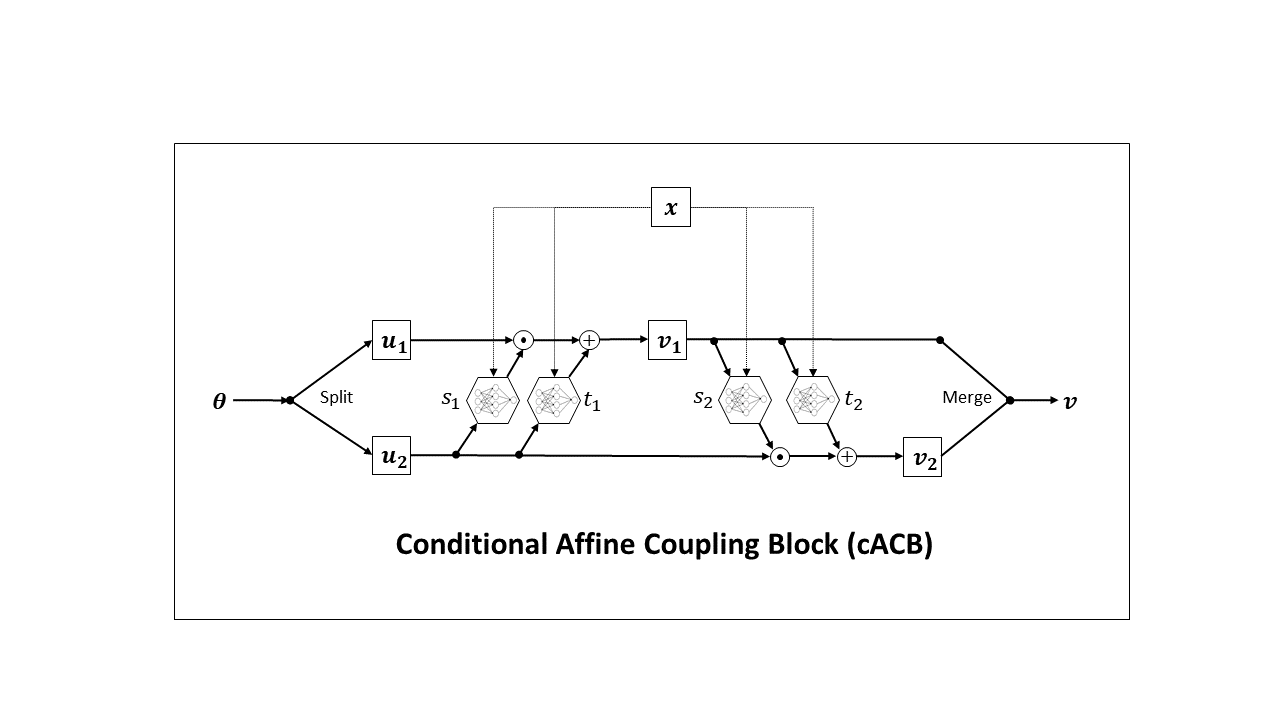
\includegraphics[width=\textwidth]{acb.png}
\caption{Second figure}
\end{figure}


%%% Add this line AFTER all your figures and tables
\FloatBarrier

\movie{Type caption for the movie here.}

\movie{Type caption for the other movie here. Adding longer text to show what happens, to decide on alignment and/or indentations.}

\movie{A third movie, just for kicks.}

\dataset{dataset_one.txt}{Type or paste caption here.}

\dataset{dataset_two.txt}{Type or paste caption here. Adding longer text to show what happens, to decide on alignment and/or indentations for multi-line or paragraph captions.}

\bibliography{references}

\end{document}